\appendix
\chapter{Plotting functions in 3D}
\section{Introduction}
In this section all the functions presented in chapter~\ref{chpt:benchmark} page~\pageref{chpt:benchmark} will be plotted in 3D.

The following graphs were generated using Matplotlib~\footnote{address} which is a python library that provides similar functionality to Matlab.

For each of the benchmark functions, the 3D graph along with the python code that was used to generate the graph will be presented.

\section{Code}
\subsection{DeJongF1 Code}
\inputminted[fontsize=\tiny]{python}{./Graphs/dejongf1.py}
\subsection{Shekel's Foxhole Code}
\inputminted[fontsize=\tiny]{python}{./Graphs/shekelsfoxhole.py}
\subsection{Rastrigin Code}
\inputminted[fontsize=\tiny]{python}{./Graphs/rastrigin.py}
\subsection{Schwefel Code}
\inputminted[fontsize=\tiny]{python}{./Graphs/Schwefel.py}
\subsection{Griewank Code}
\inputminted[fontsize=\tiny]{python}{./Graphs/Griewank.py}
\subsection{Salomon Code}
\inputminted[fontsize=\tiny]{python}{./Graphs/Salomon.py}
\subsection{Ackley Code}
\inputminted[fontsize=\tiny]{python}{./Graphs/Ackley.py}
\subsection{Six-Hump Camel Back Code}
\inputminted[fontsize=\tiny]{python}{./Graphs/Camel.py}
\subsection{Shubert Code}
\inputminted[fontsize=\tiny]{python}{./Graphs/Shubert.py}
\subsection{Himmelblau Code}
\inputminted[fontsize=\tiny]{python}{./Graphs/Himmelblau.py}
\subsection{Rosenbrock Valley Code}
\inputminted[fontsize=\tiny]{python}{./Graphs/Rosenbrock.py}
\subsection{Dropwave Code}
\inputminted[fontsize=\tiny]{python}{./Graphs/Dropwave.py}
\subsection{Easom Code}
\inputminted[fontsize=\tiny]{python}{./Graphs/Easom.py}
\subsection{Branins Code}
\inputminted[fontsize=\tiny]{python}{./Graphs/Branin.py}
\subsection{Michalewicz Code}
\inputminted[fontsize=\tiny]{python}{./Graphs/Michalewicz.py}
\subsection{Goldstein Code}
\inputminted[fontsize=\tiny]{python}{./Graphs/Goldstein.py}
\section{Graphs}
In this section 3D graphs of all the formulated functions will be presented. The 3D graphs of these functions enable one to more clearly see the problem space the algorithm is searching in.

In each of the graphs presented, on the right hand side a coloured scale is presented and the graph follows this coloured scale. The scale ranges from the maximum value to the minimum value encountered in the particular functions problem space. The maximum value in the problem space is indicated by the colour red and the minimum value in the problem space is indicated by the colour blue.

Finally the graphs are in 3 dimensions, the x and y dimensions represent any numerical number. The z dimension represents the value produce by using the function to evaluate the particular x and y coordinates.
\pagebreak
\subsection{DeJong's First Function}
~
\begin{figure}[hpt]
	\centering
	\setlength \fboxsep{0pt}
	\setlength \fboxrule{0.5pt}
	\fbox{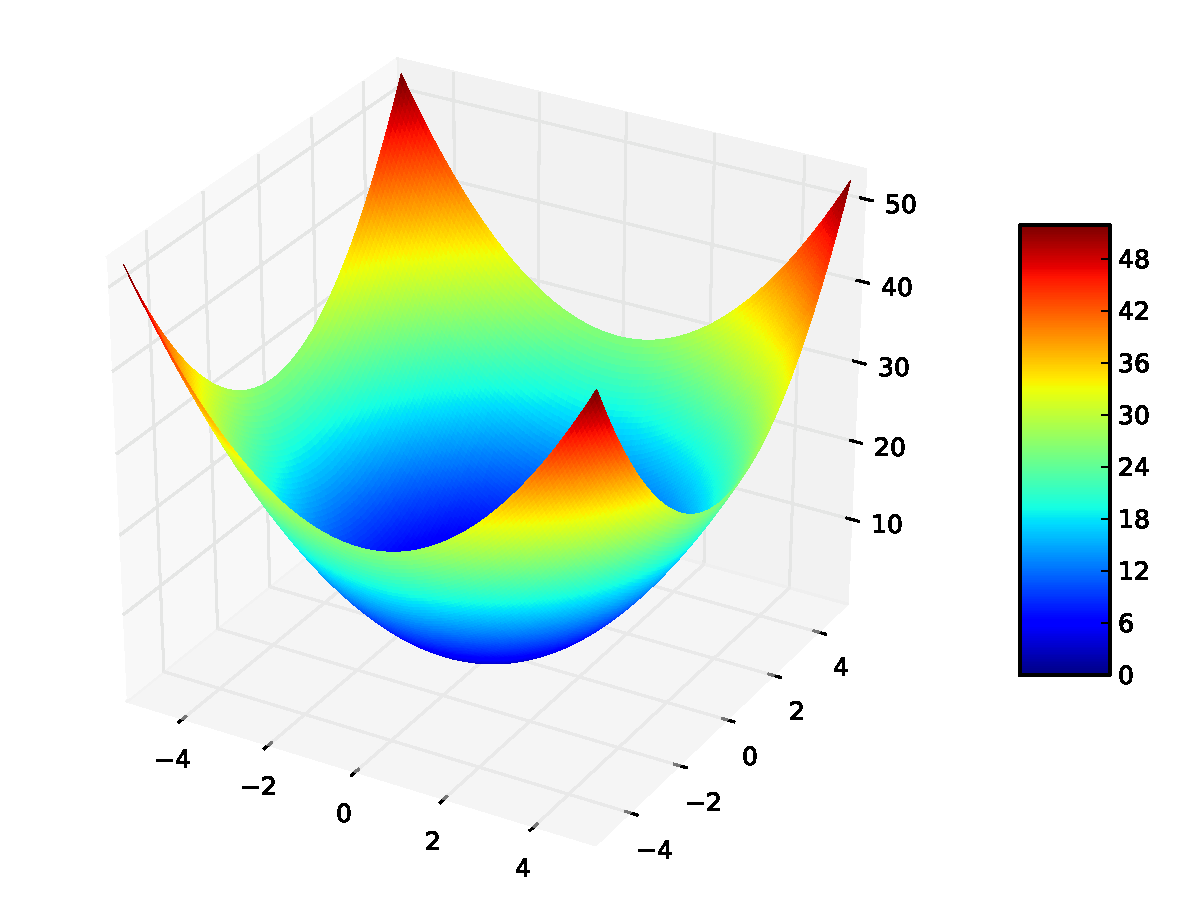
\includegraphics[width=3.0in,height=2.5in]{./Graphs/DeJongF1.pdf}}
	\caption{DeJong's First Function}
	\label{fig:DeJongF1Graph}
\end{figure}
~
\subsection{Shekel's Foxhole Function}
~
\begin{figure}[hpt]
	\centering
	\setlength \fboxsep{0pt}
	\setlength \fboxrule{0.5pt}
	\fbox{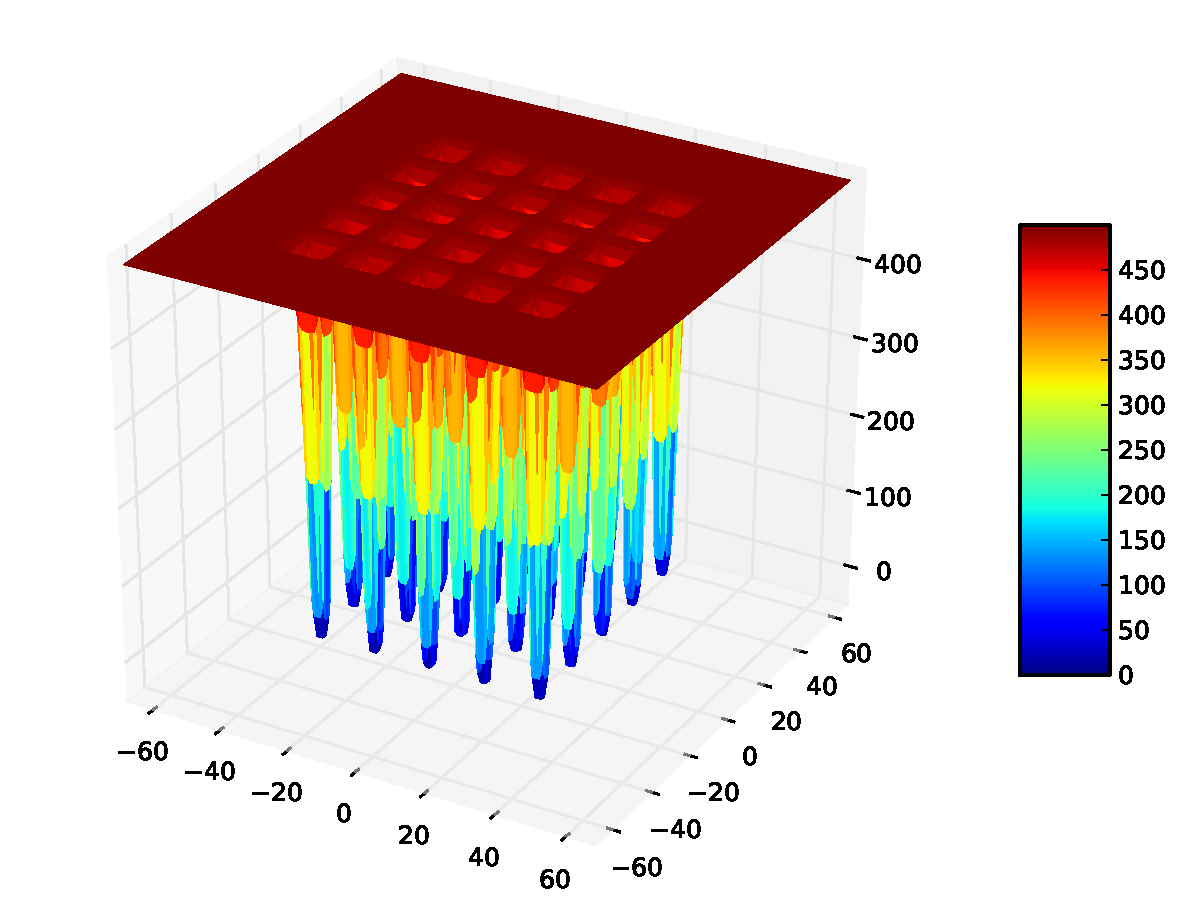
\includegraphics[width=3.0in,height=2.5in]{./Graphs/Shekel.pdf}}
	\caption{Shekel's Foxhole Function}
	\label{fig:ShekelGraph}
\end{figure}
~
\subsection{Rastrigin Function}
~
\begin{figure}[ht]
	\centering
	\setlength \fboxsep{0pt}
	\setlength \fboxrule{0.5pt}
	\fbox{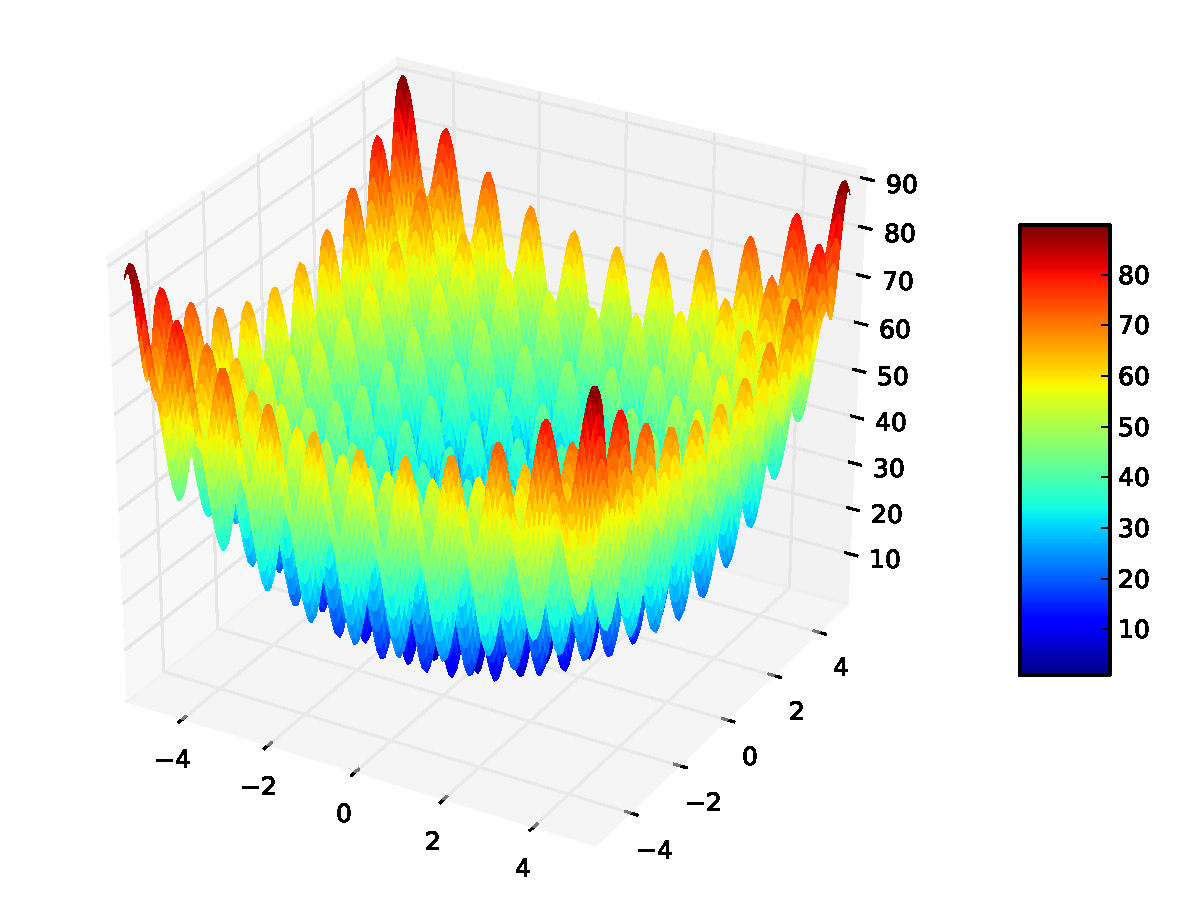
\includegraphics[width=3.0in,height=2.5in]{./Graphs/Rastrigin.pdf}}
	\caption{The Function}
	\label{fig:RastriginGraph}
\end{figure}
~
\subsection{Schwefel Function}
~
\begin{figure}[ht]
	\centering
	\setlength \fboxsep{0pt}
	\setlength \fboxrule{0.5pt}
	\fbox{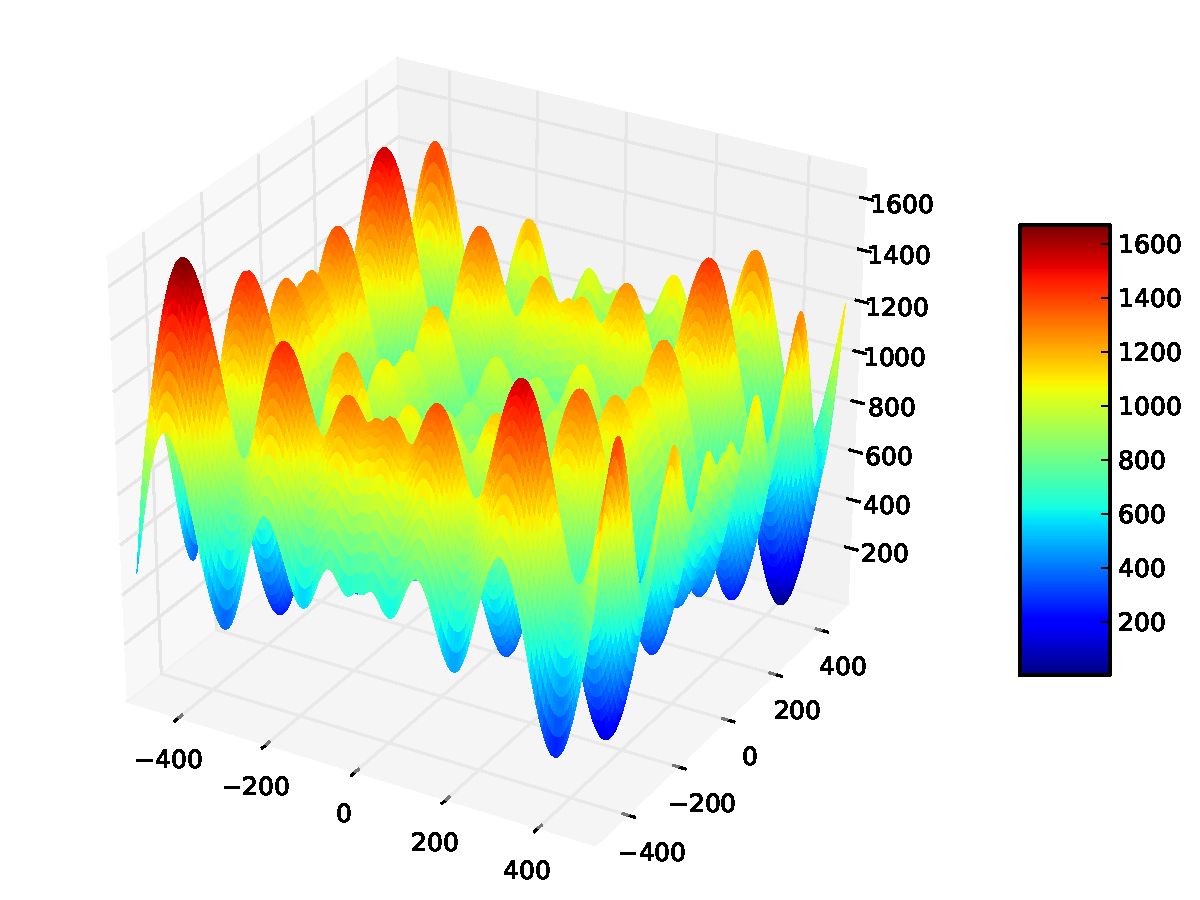
\includegraphics[width=3.0in,height=2.5in]{./Graphs/Schwefel.pdf}}
	\caption{Schwefel Function}
	\label{fig:SchwefelGraph}
\end{figure}
~
\subsection{Griewank Function}
~
\begin{figure}[ht]
	\centering
	\setlength \fboxsep{0pt}
	\setlength \fboxrule{0.5pt}
	\fbox{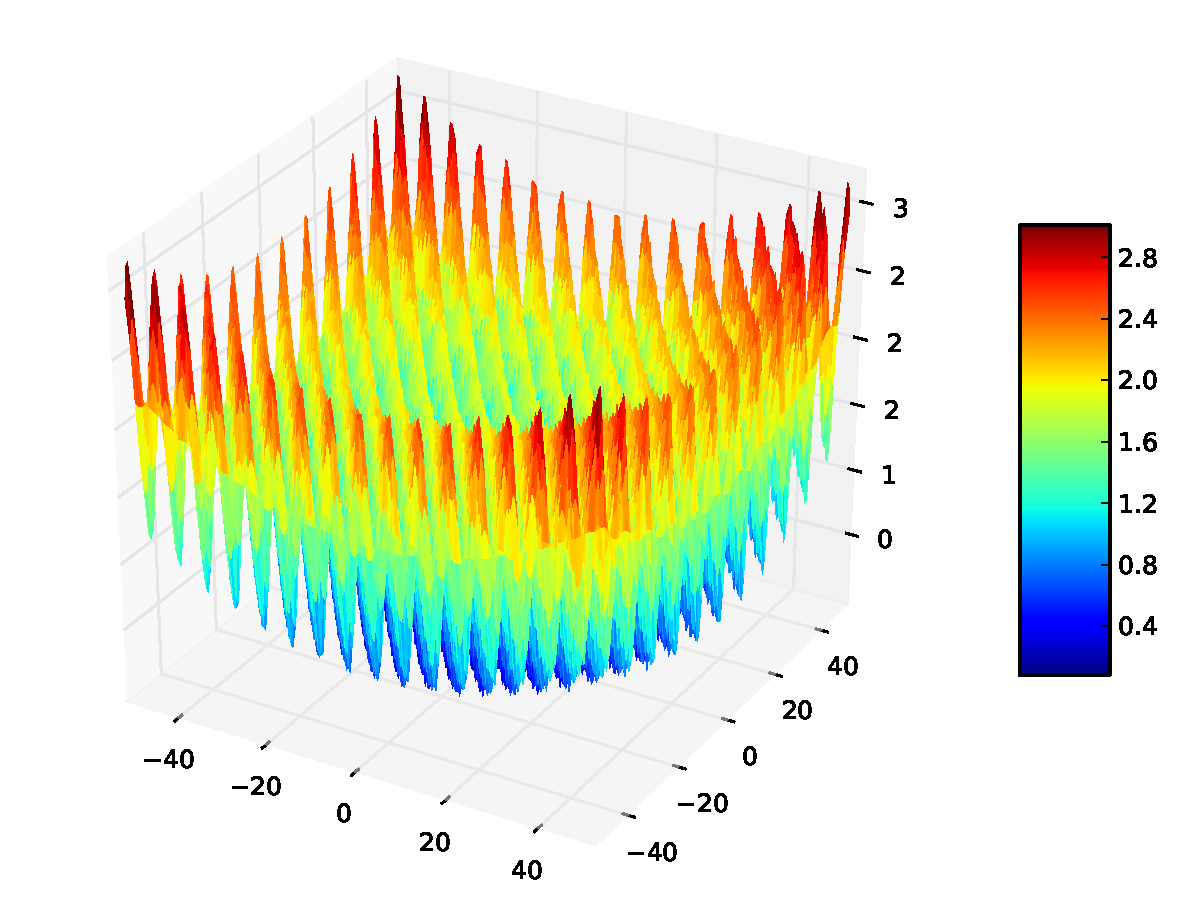
\includegraphics[width=3.0in,height=2.5in]{./Graphs/Griewank_-50_+50.pdf}}
	\caption{Griewank Function}
	\label{fig:GriewankGraph}
\end{figure}
~
\subsection{Salomon Function}
~
\begin{figure}[ht]
	\centering
	\setlength \fboxsep{0pt}
	\setlength \fboxrule{0.5pt}
	\fbox{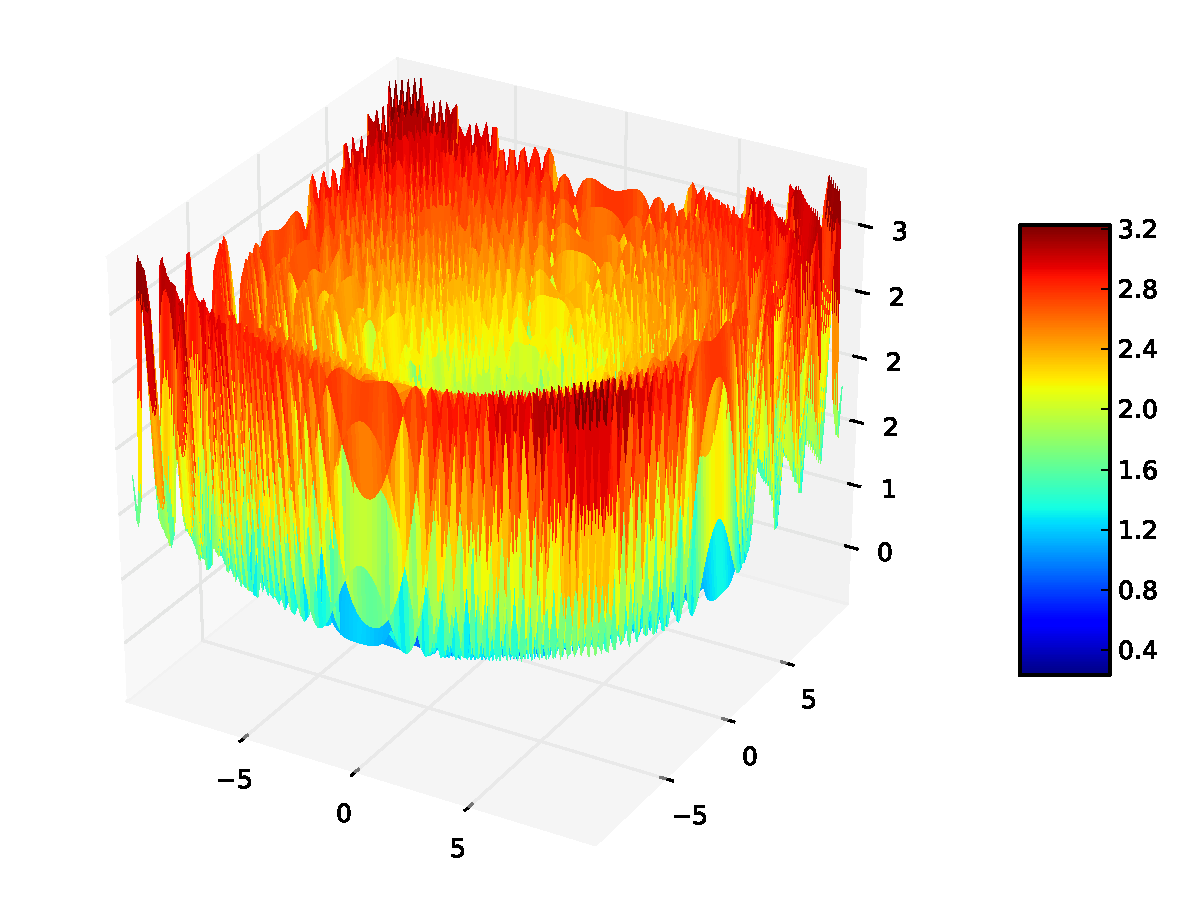
\includegraphics[width=3.0in,height=2.5in]{./Graphs/Salomon_-10_+10.pdf}}
	\caption{Salomon Function}
	\label{fig:SalomonGraph}
\end{figure}
~
\subsection{Ackley}
~
\begin{figure}[ht]
	\centering
	\setlength \fboxsep{0pt}
	\setlength \fboxrule{0.5pt}
	\fbox{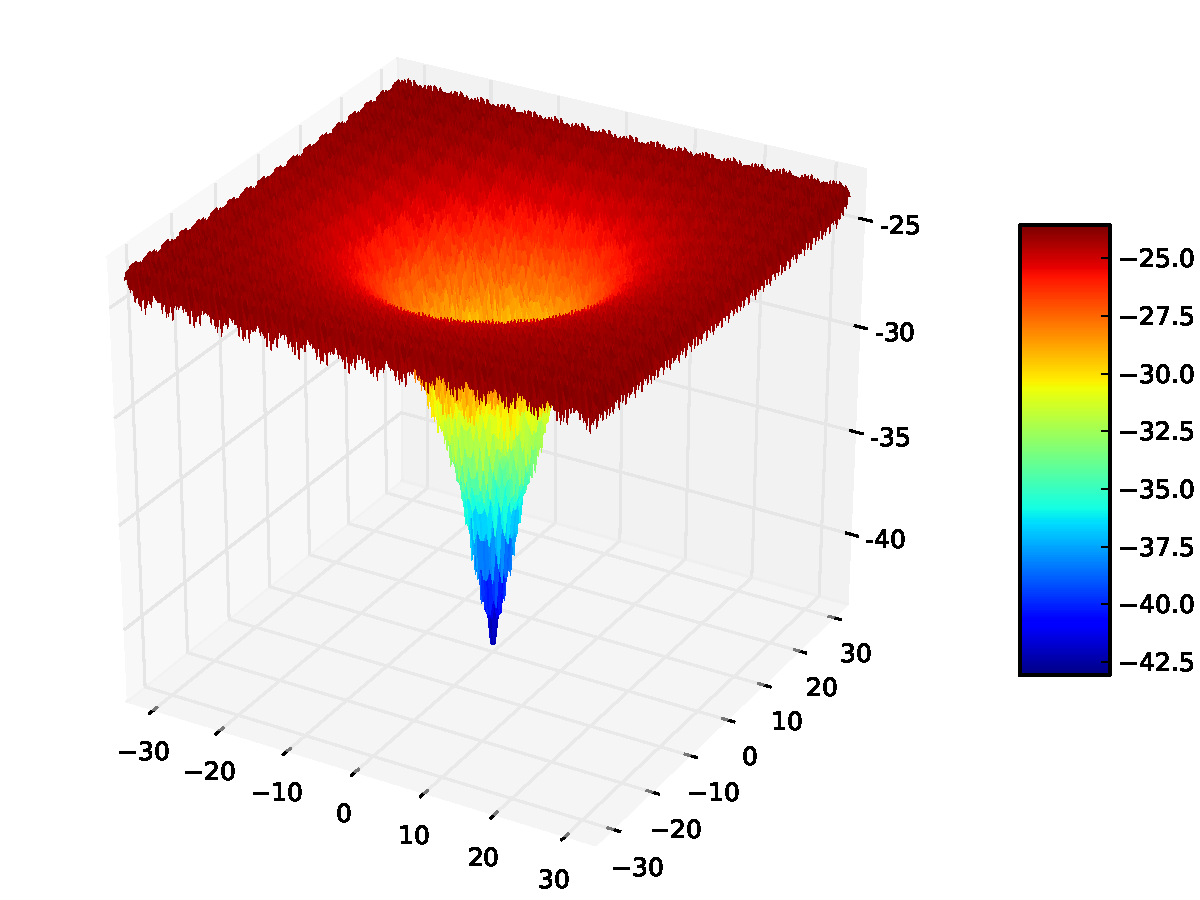
\includegraphics[width=3.0in,height=2.5in]{./Graphs/Ackley.pdf}}
	\caption{Ackley Function}
	\label{fig:AckleyGraph}
\end{figure}
~
\subsection{Six-Hump Camel Back Function}
~
\begin{figure}[ht]
	\centering
	\setlength \fboxsep{0pt}
	\setlength \fboxrule{0.5pt}
	\fbox{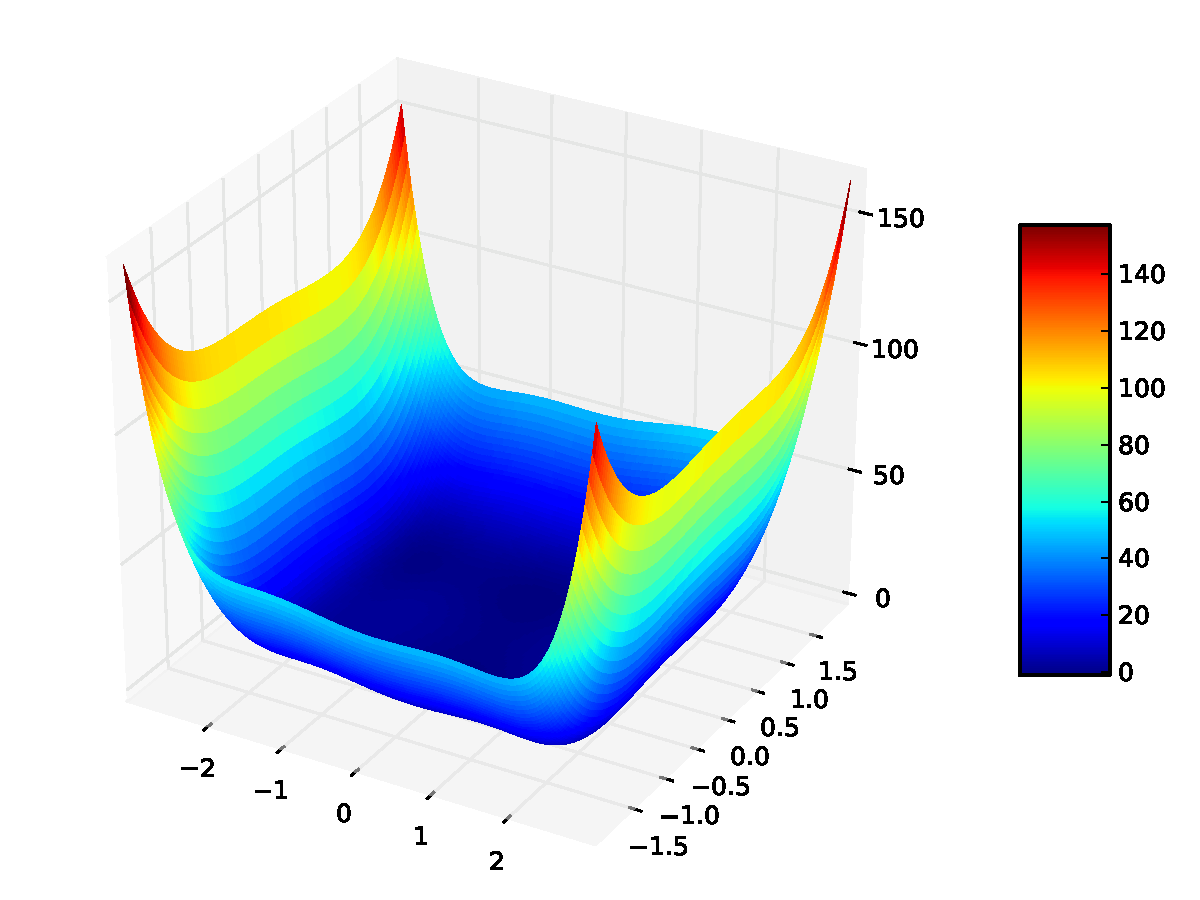
\includegraphics[width=3.0in,height=2.5in]{./Graphs/Camel.pdf}}
	\caption{Six-Hump Camel Back Function}
	\label{fig:CamelGraph}
\end{figure}
~
\subsection{Shubert Function}
~
\begin{figure}[ht]
	\centering
	\setlength \fboxsep{0pt}
	\setlength \fboxrule{0.5pt}
	\fbox{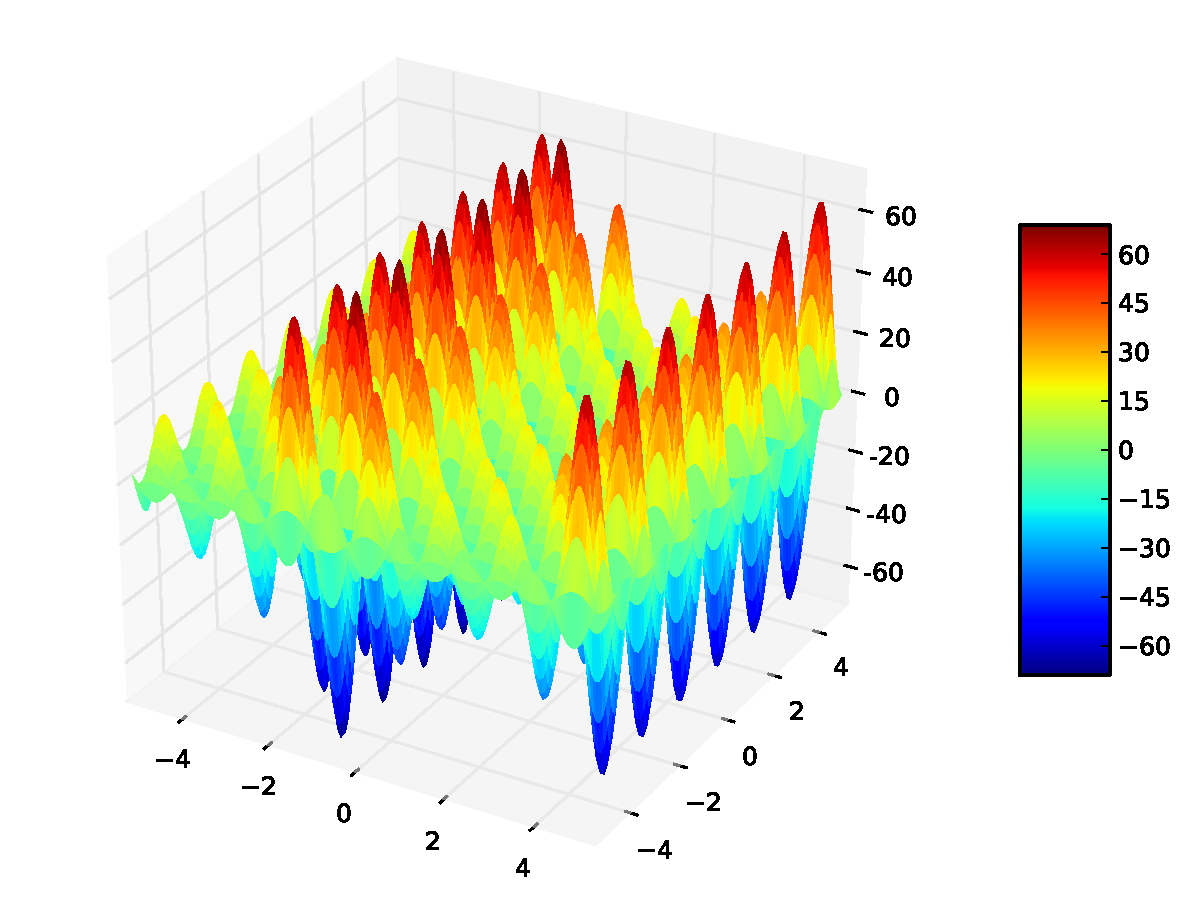
\includegraphics[width=3.0in,height=2.5in]{./Graphs/Shubert.pdf}}
	\caption{Shubert Function}
	\label{fig:ShubertGraph}
\end{figure}
~
\subsection{Himmelblau Function}
~
\begin{figure}[ht]
	\centering
	\setlength \fboxsep{0pt}
	\setlength \fboxrule{0.5pt}
	\fbox{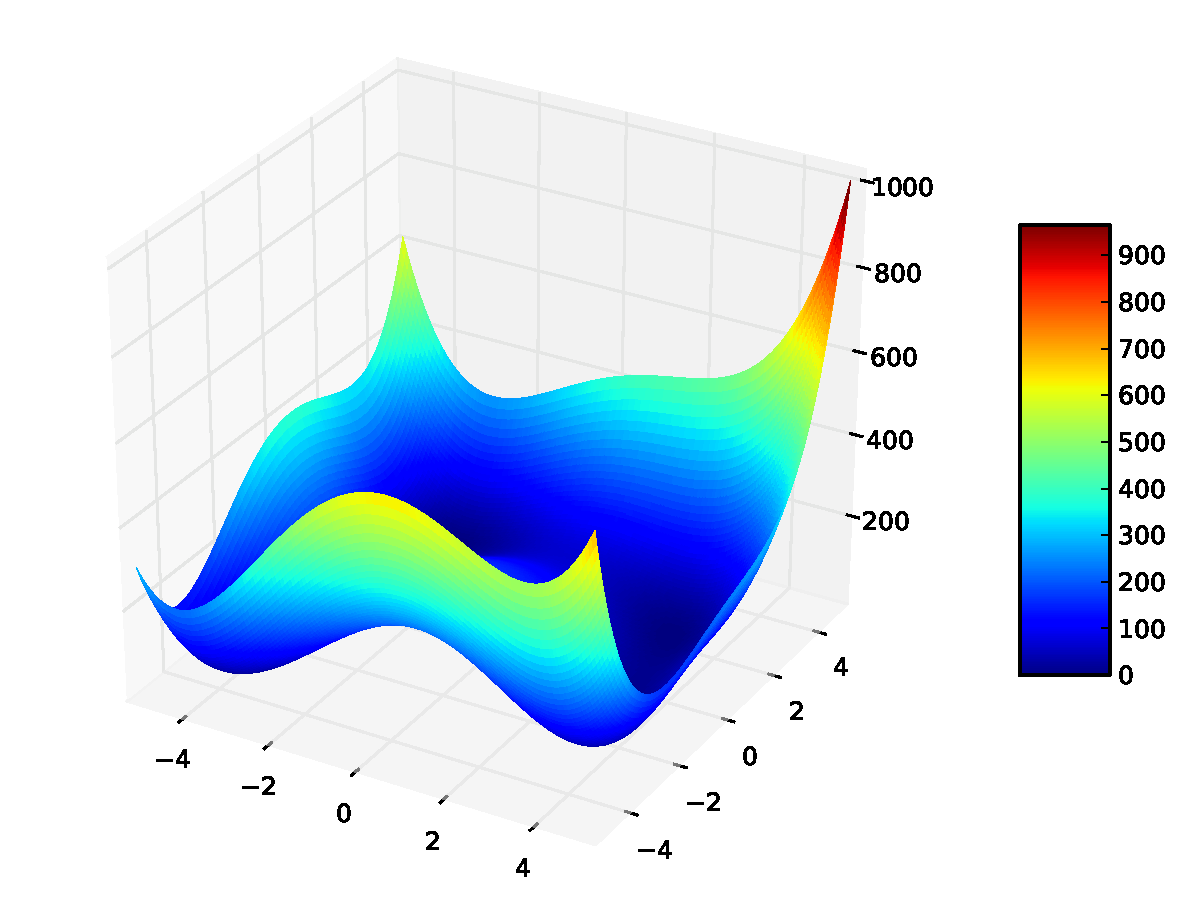
\includegraphics[width=3.0in,height=2.5in]{./Graphs/Himmelblau.pdf}}
	\caption{Himmelblau Function}
	\label{fig:HimmelblaueGraph}
\end{figure}
~
\subsection{Rosenbrock Valley Function}
~
\begin{figure}[ht]
	\centering
	\setlength \fboxsep{0pt}
	\setlength \fboxrule{0.5pt}
	\fbox{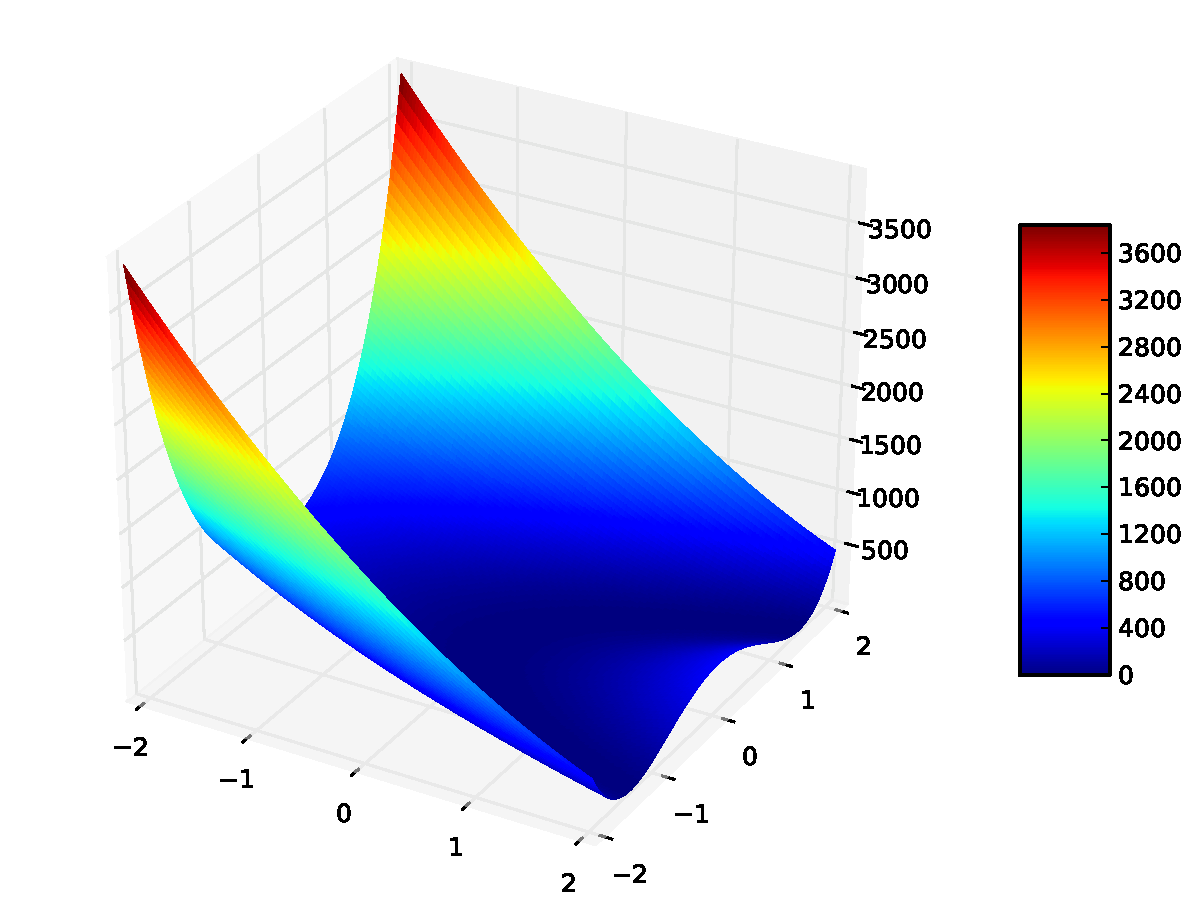
\includegraphics[width=3.0in,height=2.5in]{./Graphs/Rosenbrock.pdf}}
	\caption{Rosenbrock Valley Function}
	\label{fig:Rosenbrock}
\end{figure}
~
\subsection{Dropwave Function}
~
\begin{figure}[ht]
	\centering
	\setlength \fboxsep{0pt}
	\setlength \fboxrule{0.5pt}
	\fbox{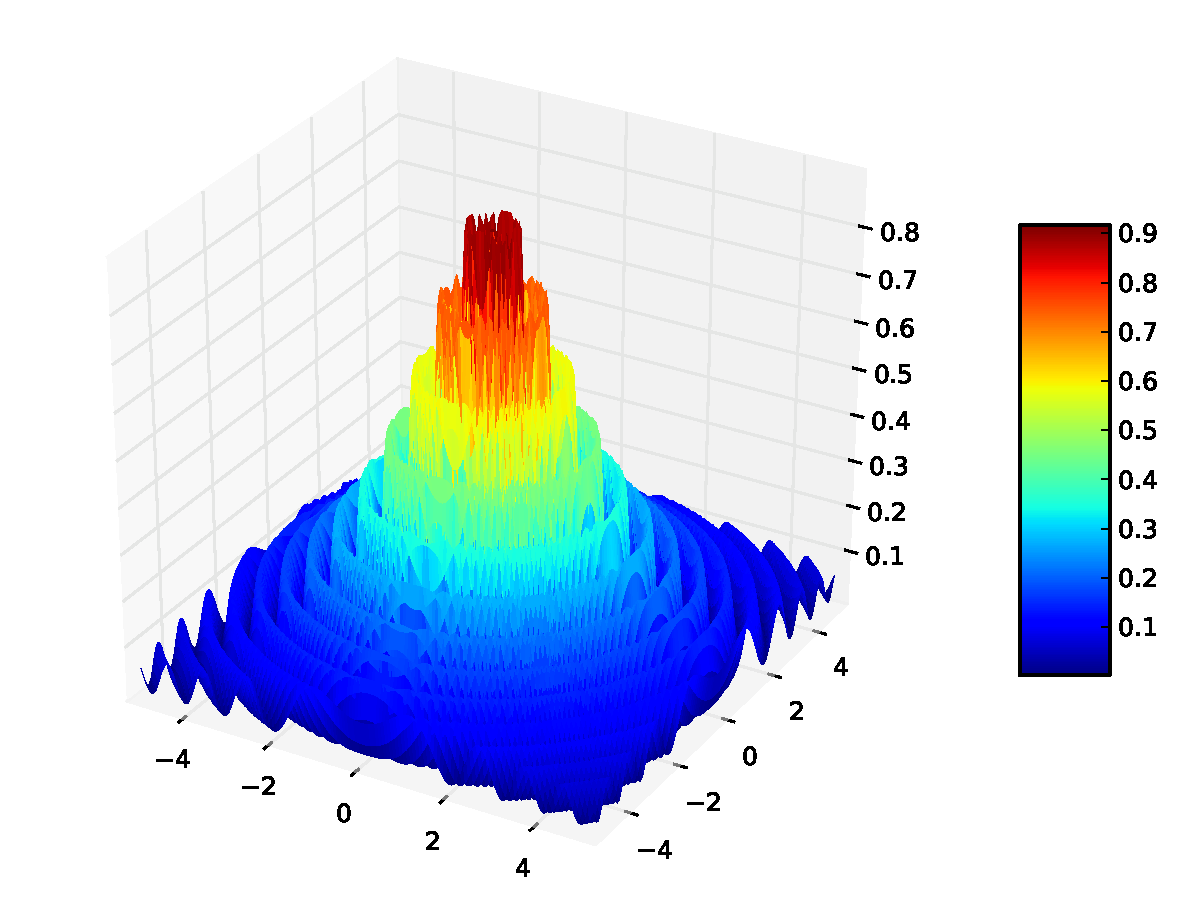
\includegraphics[width=3.0in,height=2.5in]{./Graphs/Dropwave.pdf}}
	\caption{Dropwave Function}
	\label{fig:DropwaveGraph}
\end{figure}
~
\subsection{Easom Function}
~
\begin{figure}[ht]
	\centering
	\setlength \fboxsep{0pt}
	\setlength \fboxrule{0.5pt}
	\fbox{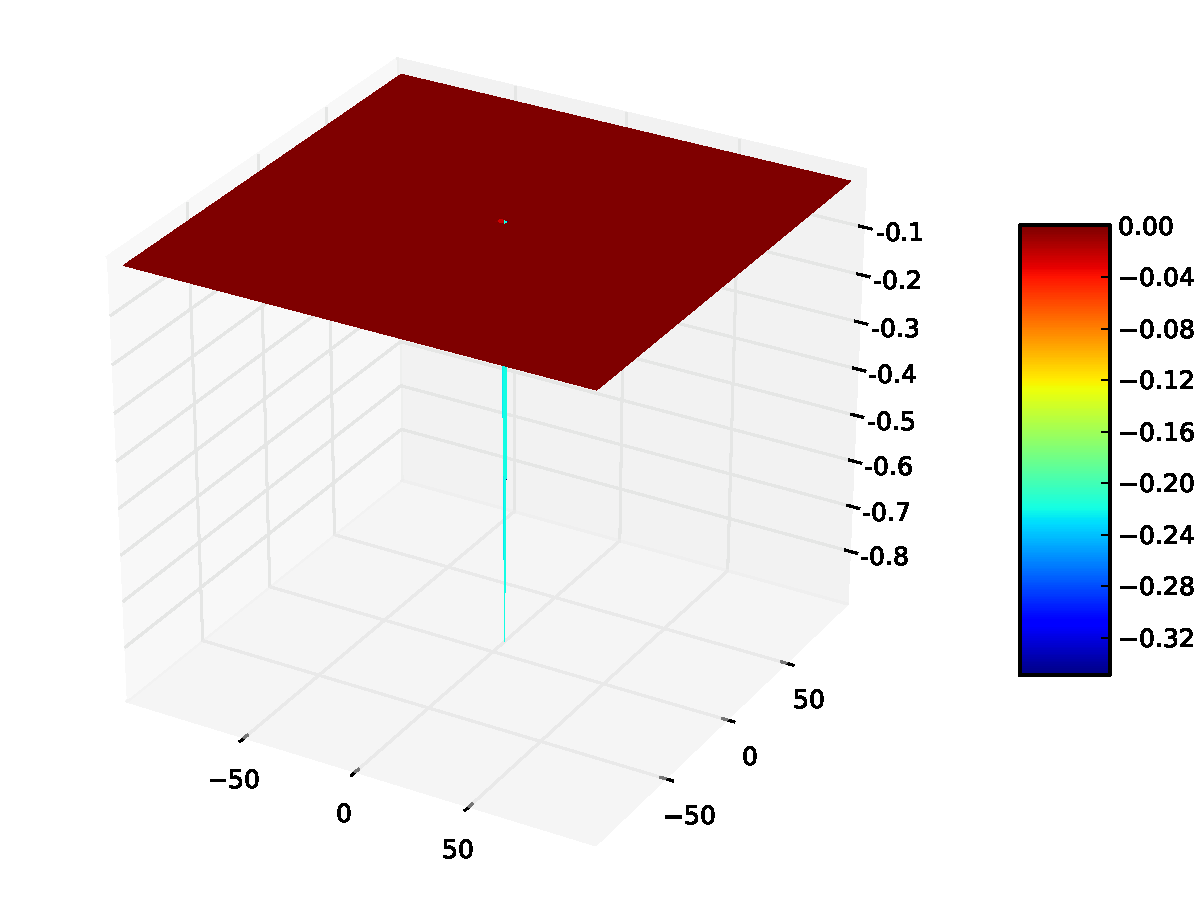
\includegraphics[width=3.0in,height=2.5in]{./Graphs/Easom_-100_+100.pdf}}
	\caption{Easom Function}
	\label{fig:EasomGraph}
\end{figure}
~
\subsection{Branin Function}
~
\begin{figure}[ht]
	\centering
	\setlength \fboxsep{0pt}
	\setlength \fboxrule{0.5pt}
	\fbox{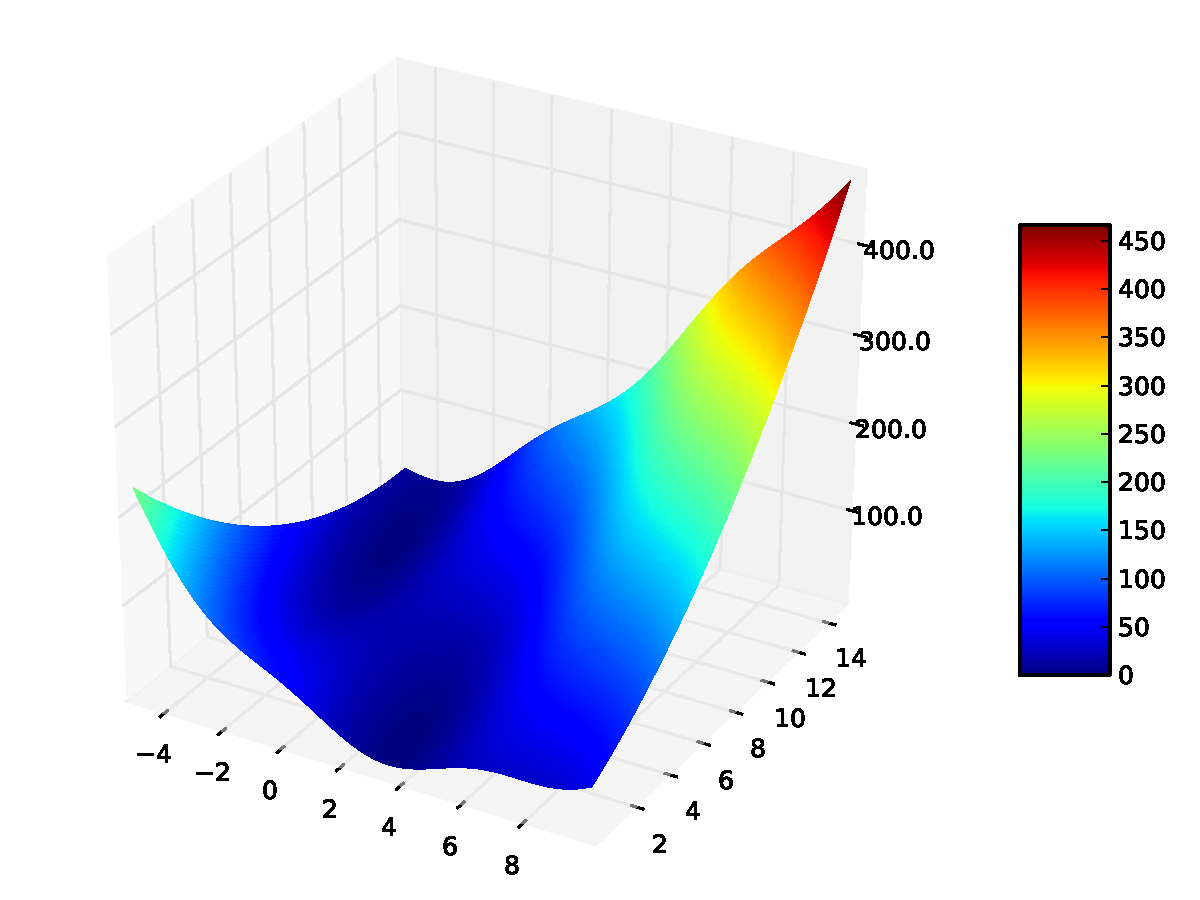
\includegraphics[width=3.0in,height=2.5in]{./Graphs/Branin.pdf}}
	\caption{Branin Function}
	\label{fig:BraninGraph}
\end{figure}
~
\subsection{Michalewicz Function}
~
\begin{figure}[ht]
	\centering
	\setlength \fboxsep{0pt}
	\setlength \fboxrule{0.5pt}
	\fbox{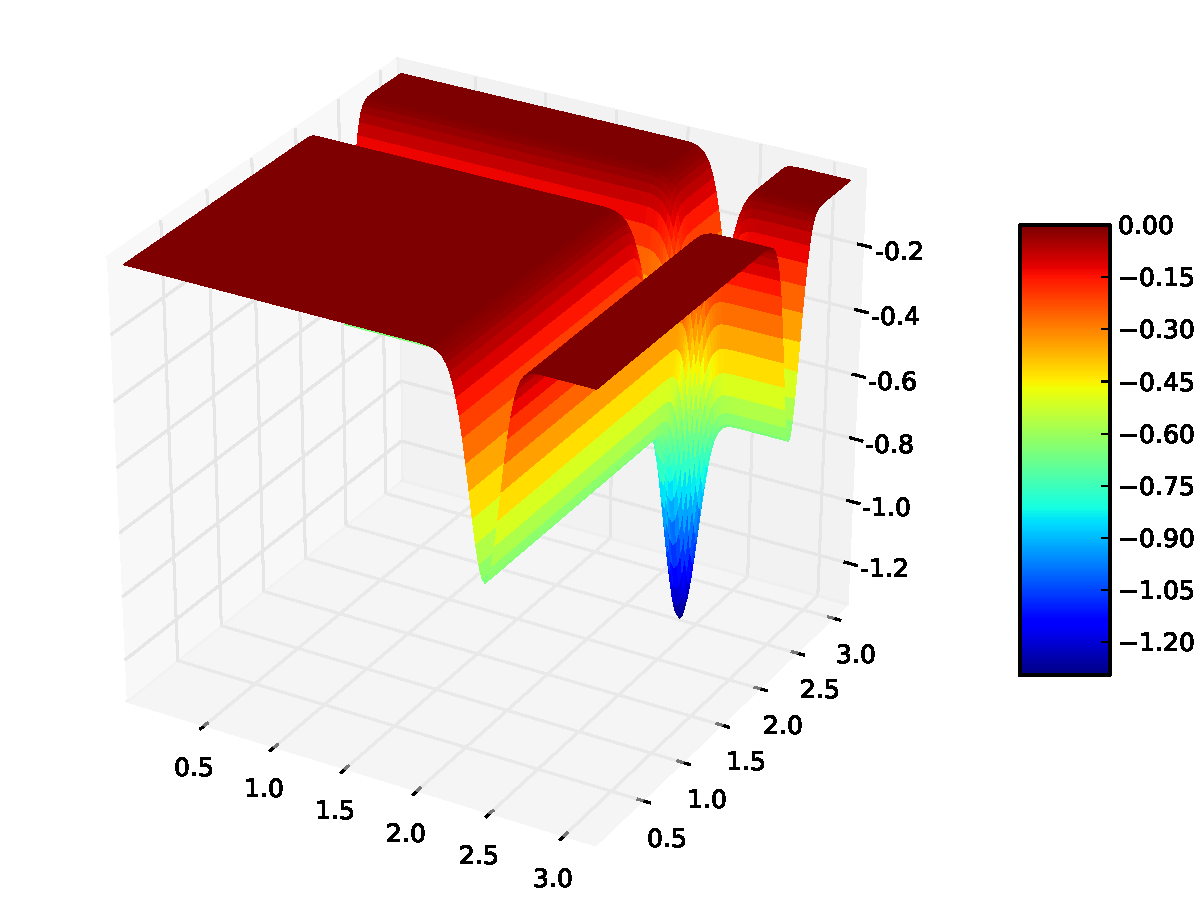
\includegraphics[width=3.0in,height=2.5in]{./Graphs/Michalewicz.pdf}}
	\caption{Michalewicz Function}
	\label{fig:MichalewiczGraph}
\end{figure}
~
\subsection{Goldstein Function}
~
\begin{figure}[ht]
	\centering
	\setlength \fboxsep{0pt}
	\setlength \fboxrule{0.5pt}
	\fbox{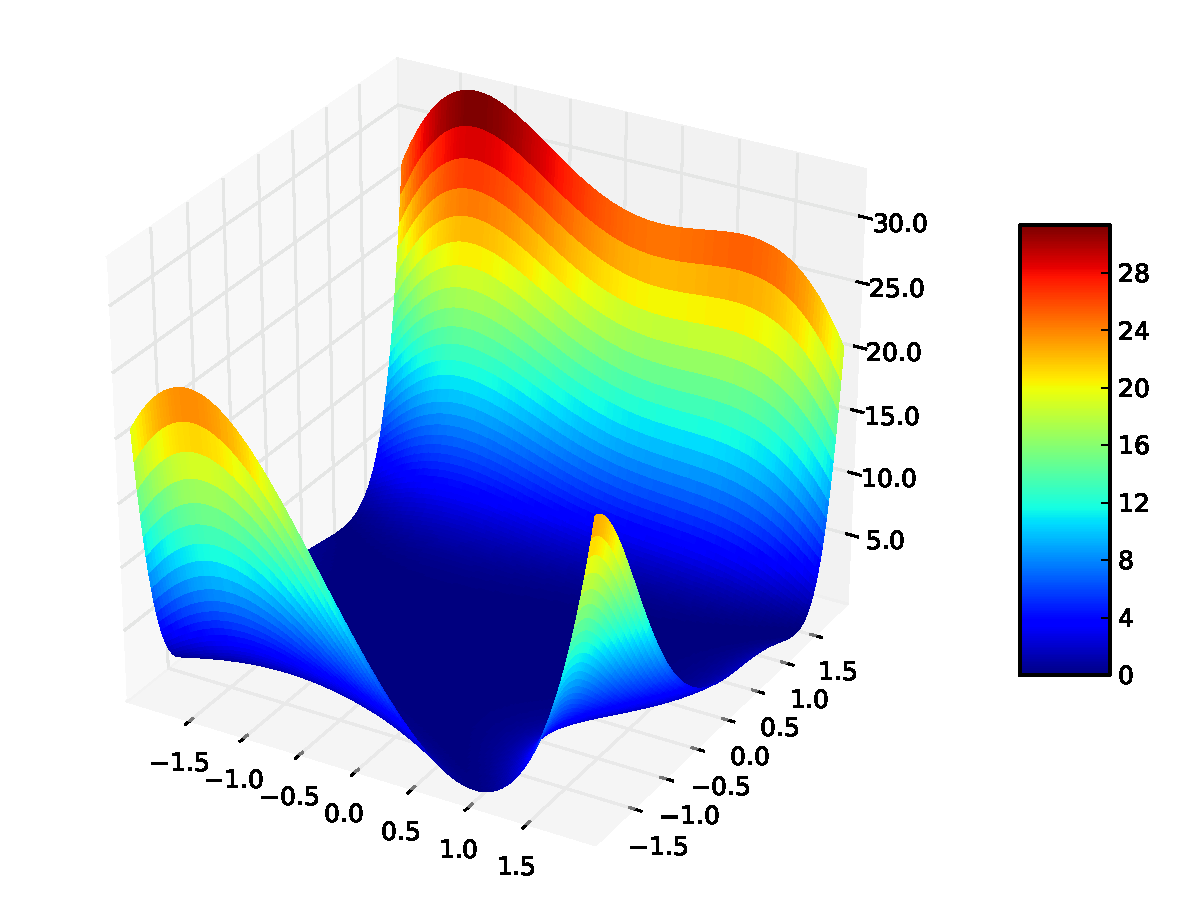
\includegraphics[width=3.0in,height=2.5in]{./Graphs/Goldstein.pdf}}
	\caption{THe Goldstein Function}
	\label{fig:GoldsteinGraph}
\end{figure}
~
